\section{Auswertung}
\subsection{Entladungsstrom}\label{sec:Entladungsstrom}
In diesem Versuchsteil soll die Abhängigkeit des Entladungsstroms  $I_{\mathrm{D}}$ von der Entladungsspannung $U_{\mathrm{D}}$, Heizstrom $I_{\mathrm{H}}$ und dem Druck $p$ untersucht werden. Dazu wird jeweils einer der Paramter variiert und die Werte der beiden anderen Paramter werden nicht verändert. Die Messung wird durchgeführt mit eingeschaltetem bzw. ausgeschaltetem  zweitem Filament in der target Kammer. Die Ergebnisse sind in den Abbildungen \ref{fig:3_1_Spannung}, \ref{fig:3_1_Strom} und \ref{fig:3_1_Druck} dargestellt. Für die Fehlerbalken sind die folgenden Fehler angenommen: $\Delta U_{\mathrm{D}} = 0.2 $ V, $\Delta I_{\mathrm{H}} = 0.02$ A, $\Delta I_{\mathrm{D}} = 0.02$ A und  $\Delta p = 0.2 $ mm. Da das Druckmessgerät kaputt war, konnte der Druck nicht gemessen werden. Der Druck ist deshalb angegeben in der Skala des Ventils, das den Gaszufluss in den Doppel Plasma Apparat regelt. Der Zusammenhang zwischen dieser Skala (in mm) und dem tatsächlichen Druck ist nicht bekannt, deshalb kann daraus der tatsächliche Druck nicht berechnet werden. Die Abhängigkeit des Entladungsstroms von der Entladungsspannung mit eingeschaltetem und ausgeschaltetem 2. Filament ist in der Abbildung \ref{fig:3_1_Spannung} dargestellt. Der konstant gehaltenne Heizstrom beträgt $ I_{\mathrm{H}} =6.00$ A für beide Sonden, für den Fall das sie eingeschaltet sind. Die Messwerte beider Messungen ähneln sich. Bei kleineren Spannungen als ca \SI{20}{V} ist der Entladungsstrom im Rahmen der Messgenauigkeit null. Bei größeren Werten kommt es erst zu einem sehr starkem Anstieg und danach ändert sich der Entladungsstrom fast nicht mehr. Der Unterscheid hervorgerufen durch das 2. Filament ist, dass mit eingeschaltetem zweitem Filament der Entladungstrom größere Werte annimmmt, bei gleicher Entladunsgspannung.  
\begin{figure}[H]
\centering
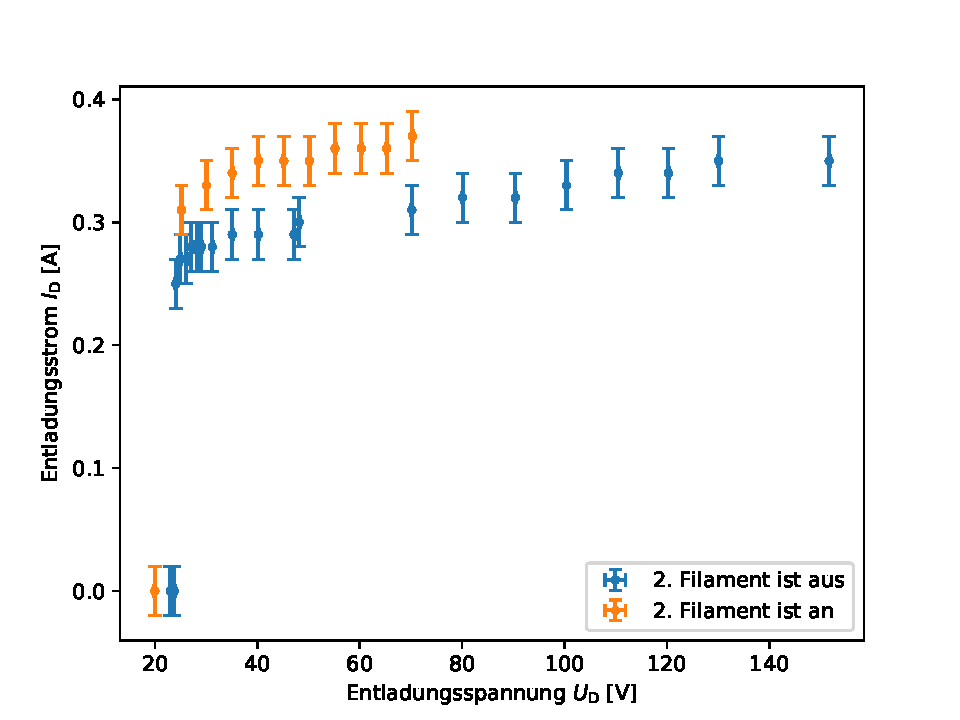
\includegraphics[scale=0.6]{3_1_Spannung.pdf}
\caption{Der Entladungstrom $I_{\mathrm{D}}$ als Funktion der Entladungsspannung $U_{\mathrm{D}}$   mit eingeschaltetem und ausgeschaltetem zweitem Filament in der target Kammer.}
\label{fig:3_1_Spannung}
\end{figure}
In der Abbildung \ref{fig:3_1_Strom} ist die Abhängigkeit des Entladungsstroms von dem Heizstrom mit eingeschaltetem und ausgeschaltete zweitem Filament dargestellt. Die konstant gehaltene Entladungsspannung beträgt $U_{\mathrm{D}}=80.3$ V in dem Fall des ausgeschaltetem zweitem Filament und  ist und $U_{\mathrm{D}}=50.3$ V für den Fall des eingeschaltetem zweitem Filament.   Die Messwerte mit eingeschaltetem und ausgeschaltetem zweitem Filament unterscheiden sich im Rahmen der Messgenauigkeit nicht voneinander. Mit steigendem Heizstrom steigt auch der Entladungsstrom an. Die Ursache dafür ist, dass aufgrund des höheren Heizstroms die Temperatur des Filaments ansteigt und somit mehr Elektronen emmitiert werden. 
\begin{figure}[H]
\centering
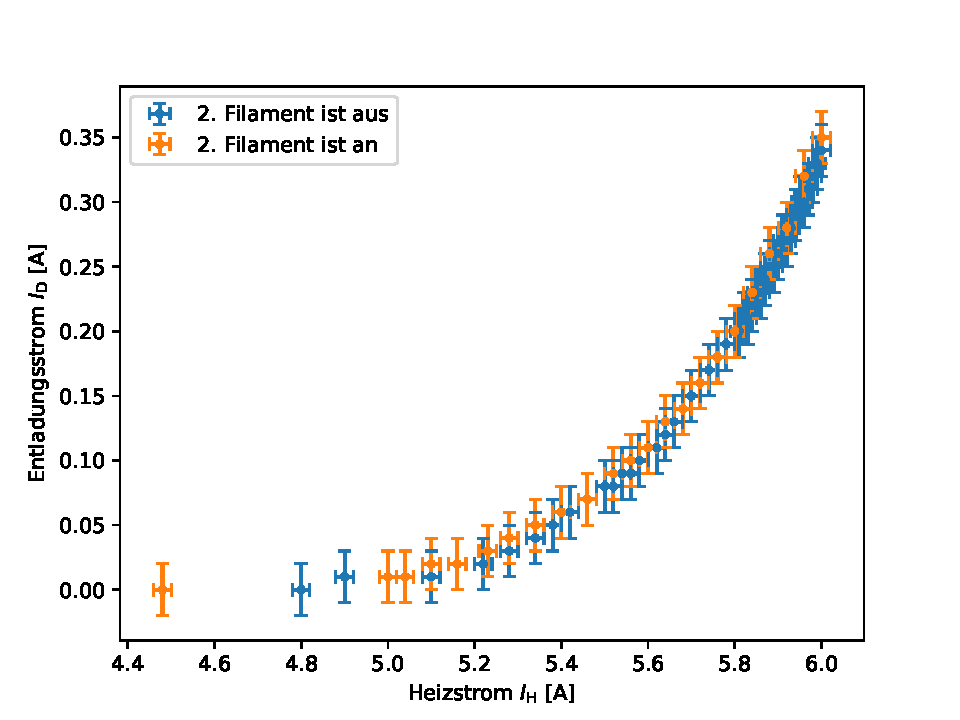
\includegraphics[scale=0.6]{3_1_Strom.pdf}
\caption{Der Entladungstrom $I_{\mathrm{D}}$ als Funktion des Heizstrom $I_{\mathrm{H}}$  mit eingeschaltetem und ausgeschaltetem zweitem Filament in der target Kammer.}
\label{fig:3_1_Strom}
\end{figure}
Der Entladungsstrom als Funktion des Druckes mit eingeschaltetem und ausgeschaltetem zweitem Filament ist in der Abbildung \ref{fig:3_1_Druck} dargestellt. Der konstant gehalteten Heizstrom beträgt $ I_{\mathrm{H}} =6.00$ A und die Entladungsspannung beträgt $U_{\mathrm{D}}=50.2$ V. In dem Bereich \SI{5}{mm} bis ca. \SI{8}{mm} gibt es nur kleine Unterschiede, zwischen eingeschaltetem und ausgeschaltetem zweitem Filament. Der Entladungsstrom steigt zunächst mit steigendem Druck an, bis bei ca. \SI{6}{mm} ein Maximum erreicht wird und sinkt danach wieder ab. Mit eingeschaltetem zweitem Filament sinkt der Entladungsstrom auch für größere Werte als \SI{8}{mm} weiter. Mit ausgeschaltetem zweitem Filament dagegen steigt der Entladungsstrom wieder an. Bei ca. \SI{9}{mm} gibt es ein Minimum im Entladungsstrom. 
\begin{figure}[H]
\centering
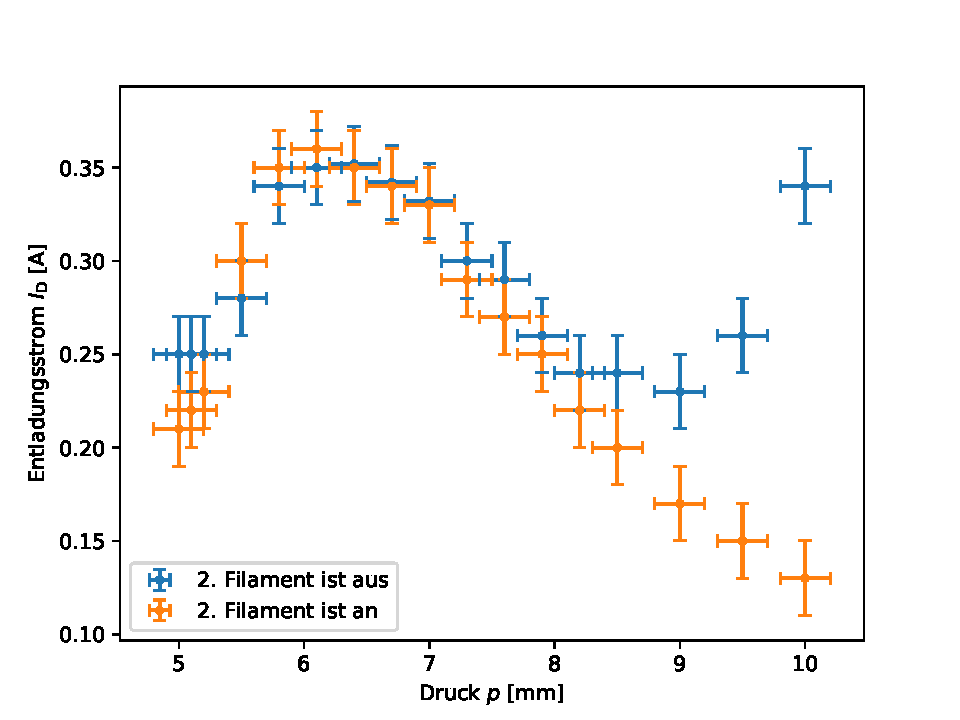
\includegraphics[scale=0.6]{3_1_Druck.pdf}
\caption{Der Entladungstrom $I_{\mathrm{D}}$ als Funktion des Druckes $p$ mit eingeschaltetem und ausgeschaltetem zweitem Filament in der target Kammer.}
\label{fig:3_1_Druck}
\end{figure}
\subsection{Plasma Oszillations Methode}
Mithilfe der Plasma  Oszillations Methode kann die Plasmadichte bestimmt werden. Die Oszillationen werden mit der Langmuir-Sonde gemessen und mit einem Spektrumanalysator dargestellt. Als erstes muss das richtige Maximum gefunden werden. Dazu müssen die Parameter variiert werden. Das Maxima das sich als einziges verändern lässt, ist das gesuchte Maximum. Die Plasmafrequenz kann dann mit dem Spektrumanalysator ermittelt werden. Zu beachten ist, das die Frequnz $f_{\mathrm{p}}$ gemessen wird, die Plasmafrequnz aber normalerweise als Kreisfrequenz angegeben wird: $\omega_{\mathrm{p}}= 2 \pi f_{\mathrm{p}}$.  Aus der Plasmafrequenz  kann dann die Plasmadichte berechnet werden:
\begin{align}
  \omega_{\mathrm{p}}=\sqrt{\frac{e^2 n}{\epsilon_0 m_{\mathrm{e}}}} = 56.5 \sqrt{n}
\end{align}
Durch Umstellen der Gleichung erhält man
\begin{align}
  n=\left( \frac{\omega_{\mathrm{p}}}{56.5} \right)^2=\left( \frac{2 \pi f_{\mathrm{p}}}{56.5} \right)^2.
 \end{align}
Der Fehler kann durch Fehlerfortpfalnzung berechnet werden, wobei als Fehler der gemessenen Frequenz  $\Delta f= 5$ MHz angenommen wird.  
\begin{align}
  \Delta n &= \frac{\mathrm{d} n}{\mathrm{d} f} \Delta f \\
  &=\left( \frac{2 \pi}{56.5} \right)^2 2 f_{\mathrm{p}} \Delta f
\end{align}
Analog zum Kapitel \ref{sec:Entladungsstrom} wird die Abhängigkeit der Plasmadichte von den Parametern Entladungsspannung, Heizstrom und Druck bestimmt. Die Plasmadichte als Funktion der Entladungsspannung ist in der Abbildung \ref{fig:3_2_Spannung} dargestellt. Die Plasmadichte steigt mit steigender Entladungsspannung an. Bei ca. \SI{80}{A} Entladungsspannung kommt es zu eienm Sattelpunkt. Danach steigt die Plasmadichte wieder an. 
\begin{figure}[H]
\centering
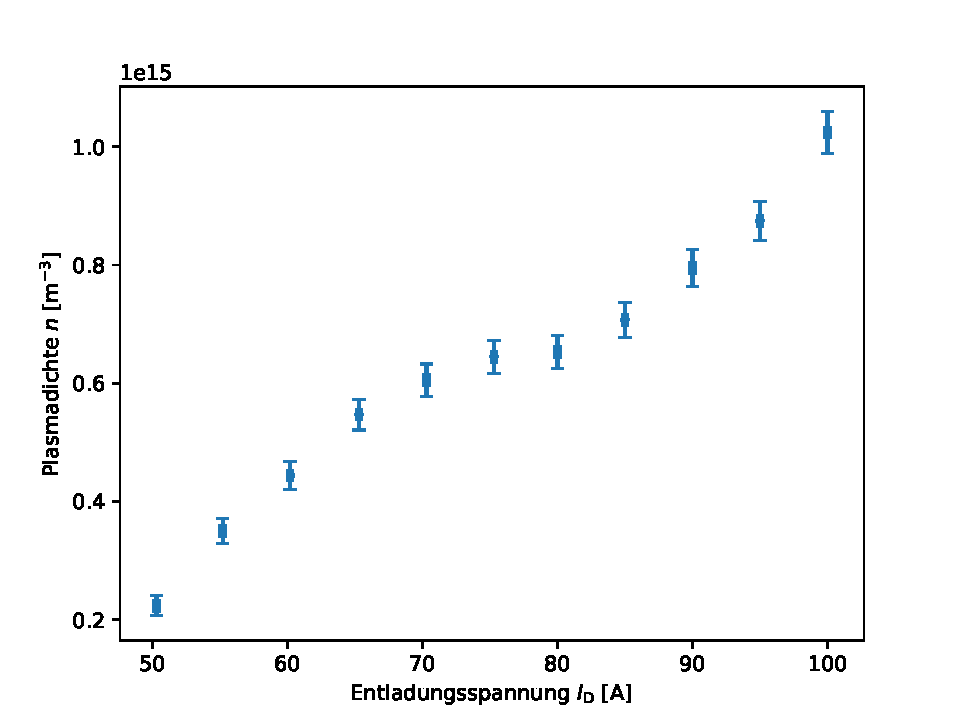
\includegraphics[scale=0.6]{3_2_Spannung.pdf}
\caption{Die Plasmadichte  als Funktion der Entladungsspannung.}
\label{fig:3_2_Spannung}
\end{figure}
Die Plasmadichte als Funktion des Heizstroms ist in der Abbildung \ref{fig:3_2_Strom} dargestellt. Zu erkennen ist  näherungsweise ein linearer Zusammenhang zwischen dem Heizstrom und der Plasmadichte.  
\begin{figure}[H]
\centering
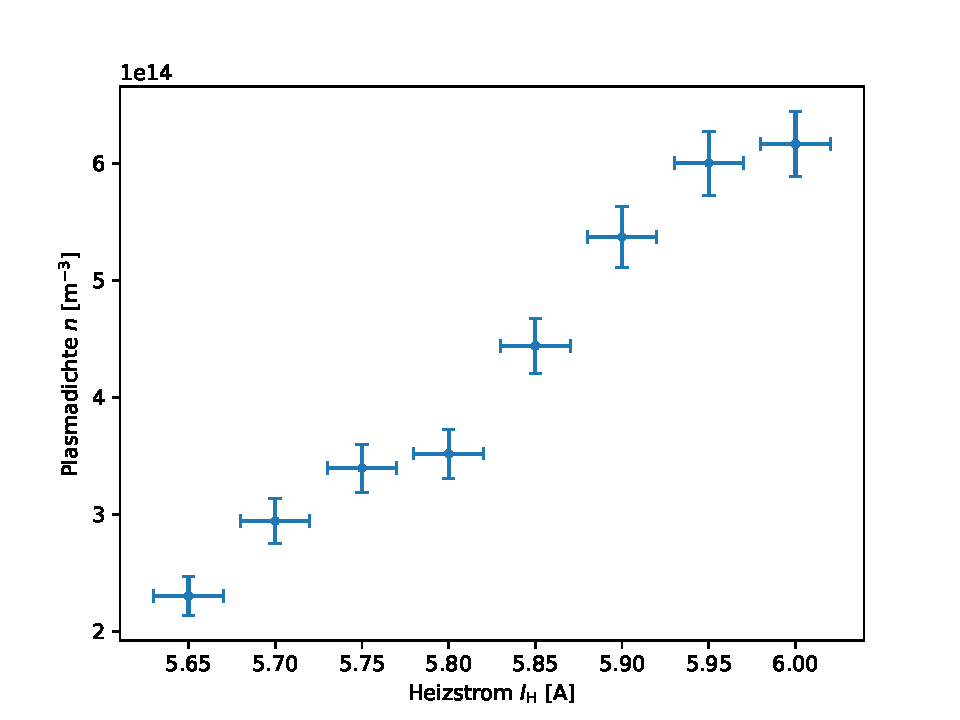
\includegraphics[scale=0.6]{3_2_Strom.pdf}
\caption{Die Plasmadichte als Funktion des Heizstroms.}
\label{fig:3_2_Strom}
\end{figure}
Die Plasmadichte in Abhängigkeit des Druckes ist in der Abbildung \ref{fig:3_2_Druck} dargestellt. Die Plasmadichte ist bis ca. \SI{5}{mm} fast konstant. Danach gibt es einen sehr starken Anstieg. Ob dieser Verlauf den Zusammenhang zwischen Druck und Plasmadichte korrekt beschreibt kann nicht untersucht werden, da wie bereits erwähnt das Druckmessgerät kaputt ist. 
\begin{figure}[H]
\centering
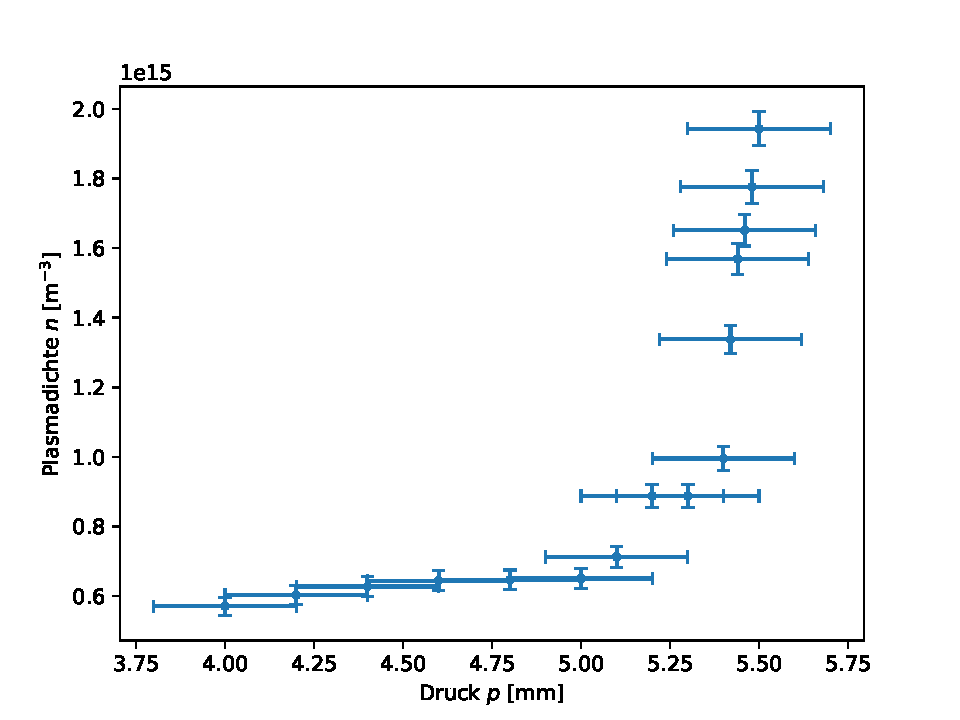
\includegraphics[scale=0.6]{3_2_Druck.pdf}
\caption{Die Plasmadichte als Funktion des Drucks.}
\label{fig:3_2_Druck}
\end{figure}
In allen drei Diagrammen für die Plasmadichte  \ref{fig:3_2_Spannung}, \ref{fig:3_2_Strom} und  \ref{fig:3_2_Druck} liegt die Plasmadicht immer im Bereich von $n=10^{14}\ \frac{1}{\mathrm{m}^3}$ bis  $n=10^{15}\ \frac{1}{\mathrm{m}^3}$.
\subsection{Ionen Akustikwellen}
Die Dispersionsrelation einer Ionen Akustikwelle kann durch eine Anregung mit einer sinusförmige Spannung am Gitter gemessen werden. Gemessen wird mittels einer Langmuir Sonde die Wellenlänge $\lambda$ und die dazugehörige Frequenz $f$. Aus der Wellenlänge kann der Wellenvektor $k$ und aus der Frequnz die Kreisfrequenz  $\omega$ berechnet werden.
\begin{align}
  \omega & = 2 \pi f \\
  k & = \frac{2 \pi}{\lambda}
\end{align}
Der Fehler $\Delta k$ wird mittels Fehlerfortpflanzung berechnet, wobei für die Wellenlänge $\Delta \lambda=0.1$ cm angenommen wird.
\begin{align}
  \Delta k = \bigl| \frac{\mathrm{d} k}{\mathrm{d} \lambda} \bigl| \Delta \lambda = \frac{2\pi}{\lambda^2} \Delta \lambda
\end{align}
Für die Bestimmung der Schallgeschwindigkeit kann die  Funtkion 
\begin{align}
  \omega(k) = \sqrt{\frac{T_{\mathrm{e}} + 3 T_{\mathrm{i}}}{m_{\mathrm{i}}}} k = c_{\mathrm{s}} k
  \label{eq:Dispersion_3_3}
\end{align}
zum fitten benutzt werden, wobei $T_{\mathrm{e}}$ die Temperatur der Elektronen, $T_{\mathrm{i}}$ die Temperatur der Ionen, $m_{\mathrm{i}}$ die Masse der Ionen und $c_{\mathrm{s}}$ die Schallgeschwindigkeit ist. Das bedeutet durch das Fitten mir einer Geraden
\begin{align}
  f(x)= a x +b
  \label{eq:fit_Dispersion}
\end{align}
kann die Schallgeschwindigkeit und daraus dann die Elektronentemperatur bestimmt werden. Die Messung wurde für drei unterschiedliche Drücke durchgeführt und die Ergebisse sind in der Abbildung \ref{fig:3_3_Dispersion} dargestellt.
\begin{figure}[H]
\centering
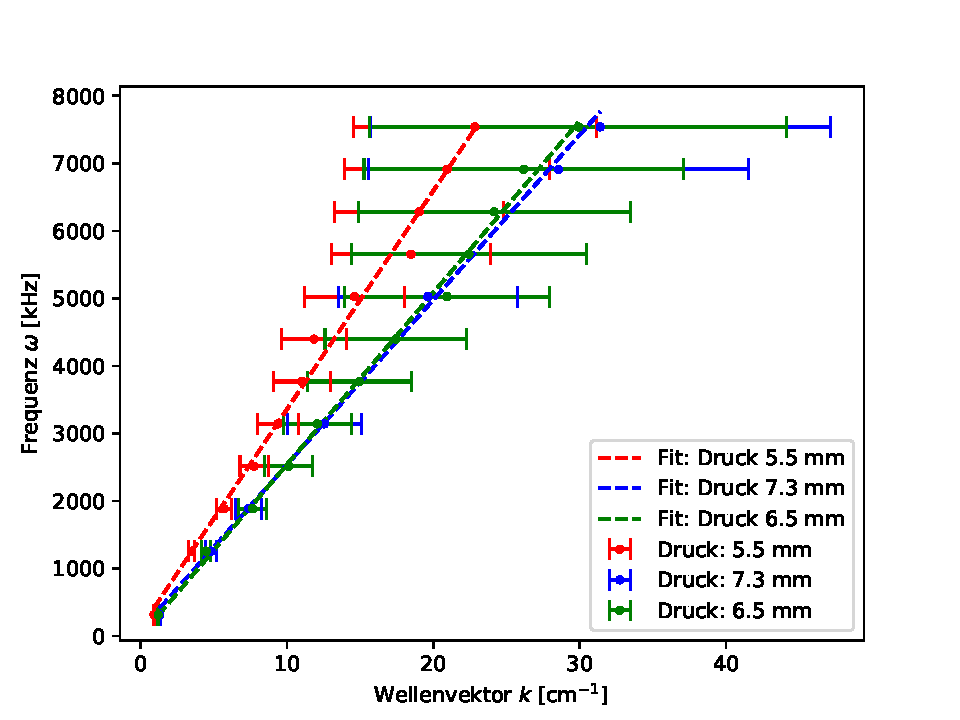
\includegraphics[scale=0.6]{3_3_Dispersion.pdf}
\caption{Die Dispersionsrelation für Ionen Akustikwellen für unterschiedliche Drücke mit eingezeichneten Fitfunktionen.}
\label{fig:3_3_Dispersion}
\end{figure}
Die Schallgeschwindigkeit entspricht in der Gleichung \eqref{eq:fit_Dispersion} dem Parameter a. Für die drei unterschiedlichen Drücke in Abbildung \ref{fig:3_3_Dispersion} ergeben sich die folgenden Werte:
\begin{align}
  a_1 & = 3236.29\  \mathrm{m s}^{-1} \\
  a_2 & = 2443.43\  \mathrm{m s}^{-1} \\
  a_3 & = 2544.33\  \mathrm{m s}^{-1}
\end{align}
Der Mittelwert dieser drei Werte ergibt die Schallgeschwindigkeit
\begin{align}
  c_{\mathrm{s}}= 2741.35\  \mathrm{m s}^{-1}.
  \label{eq:Wert_Schallgeschwindigkeit}
\end{align}
Aus der Schallgeschwindigkeit kann mit der Gleichung \eqref{eq:Dispersion_3_3} die Elekronentemperatur berechnet werden. Durch Vervendung von  $T_{\mathrm{e}} \gg T_{\mathrm{i}}$ vereinfacht sich die Gleichung  \eqref{eq:Dispersion_3_3} zu
\begin{align}
  T_{\mathrm{e}} \approx m_{\mathrm{i}} c_{\mathrm{s}}^2,
  \end{align}
wobei $ m_{\mathrm{i}}=6.6334 \cdot 10^{-26}$ kg die Atommasse von Argon ist. Mit dieser Masse und der Schallgeschwindigkeit aus \eqref{eq:Wert_Schallgeschwindigkeit} ergibt sich
\begin{align}
   T_{\mathrm{e}} \approx m_{\mathrm{i}} c_{\mathrm{s}}^2= 3.1108\ \mathrm{eV}.
  \end{align} 
Daraus lässt sich die tatsächliche Temperatur $T=T_{\mathrm{e}}/k_{\mathrm{B}}=3.809 \cdot 10^4$ K bestimmen.  Um die Dämpfung zu bestimmen, kann die Amplitude für unterschiedliche Positionen untersucht werden. Die Amplituden nehmen exponentiell mit dem Abstand ab
\begin{align}
  A(x) = A(x=0) \mathrm{exp}\ \left(- \frac{x}{\lambda_{\mathrm{damp}}}  \right),
  \label{eq:Damp_allgemein}
\end{align}
wobei $\lambda_{\mathrm{damp}}$ die Dämpfungslänge ist. Ermittelt werden kann diese durch Fitten der Gleichung \eqref{eq:Damp_allgemein} an die Messwerte. Dies ist für drei unterschiedliche Drücke gemacht worden und die Ergebniss sind in der Abbildung \ref {fig:3_3_Daempfung} dargestellt. 
\begin{figure}[H]
\centering
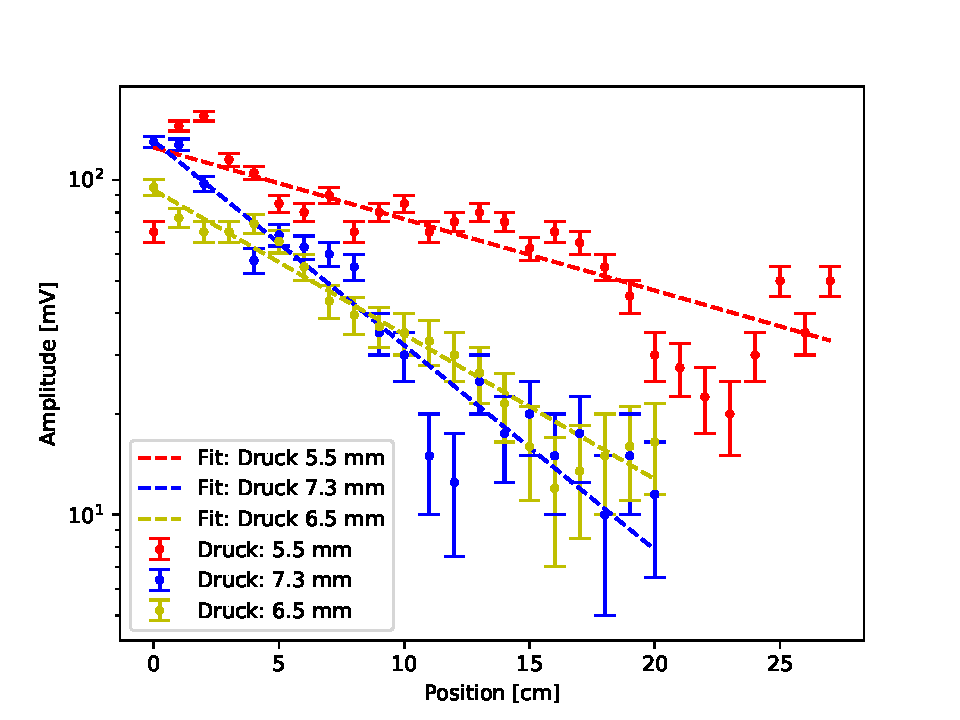
\includegraphics[scale=0.6]{3_3_Daempfung.pdf}
\caption{Die Dämpfung für Ionen Akustikwellen für unterschiedliche Drücke mit eingezeichneten Fitfunktionen.}
\label{fig:3_3_Daempfung}
\end{figure}
Die durch fitten ermittelten Dämpfungslängen sind
\begin{align}
  \lambda_{\mathrm{damp} 1} &= 20.348\ \mathrm{cm} \\
  \lambda_{\mathrm{damp} 2} &=  7.962\  \mathrm{cm} \\
  \lambda_{\mathrm{damp} 3} &= 10.059\  \mathrm{cm}. 
\end{align}  
\subsection{Schock Wellen}
Wird die Amplitude der Spannung am Gitter erhöht, kommt es zu einem Übergang von linearen Ionen Akustikwellen zu nicht linearen Schockwellen.  Dieser Übergang ist mit einem Oszilloskop gemessen worden. Die gemessen Daten sind in den Abbildungen \ref{fig:oszi_2}, \ref{fig:oszi_1} und \ref{fig:oszi_3} dargestellt. Die blaue Kurve ist jeweils das gemessene Signal und die andere Kurve die am Gitter angelegte Spannung. Gut zu erkennen ist, das mit steigender Amplitude der Spannung am Gitter, das gemessene Signal immer weniger wie eine Sinus-Funktion aussieht. 
\begin{figure}[H]
\centering
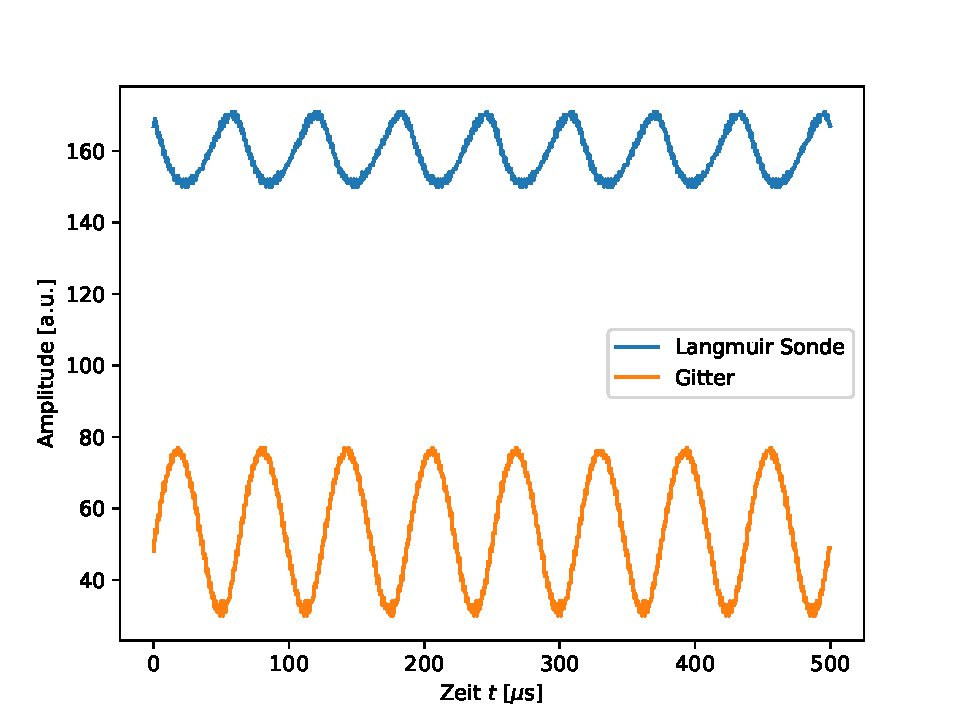
\includegraphics[scale=0.6]{oszi_2.pdf}
\caption{Die angelegte Spannung am Gitter und das gemessene Signal mit der Langmuir-Sonde.}
\label{fig:oszi_2}
\end{figure}

\begin{figure}[H]
\centering
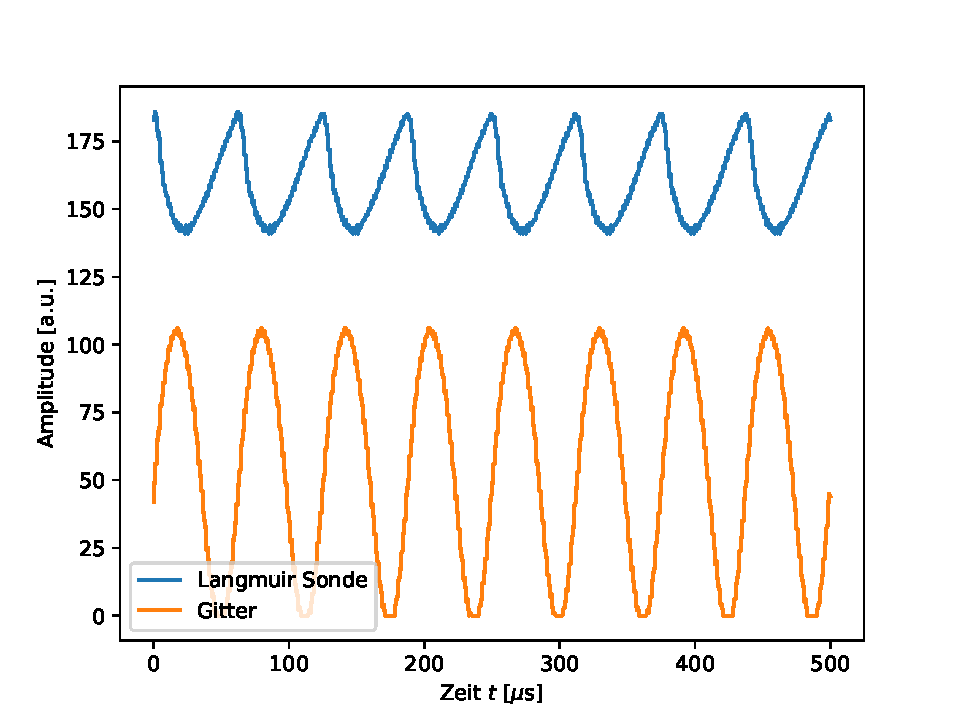
\includegraphics[scale=0.6]{oszi_1.pdf}
\caption{Die angelegte Spannung am Gitter und das gemessene Signal mit der Langmuir-Sonde.}
\label{fig:oszi_1}
\end{figure}



\begin{figure}[H]
\centering
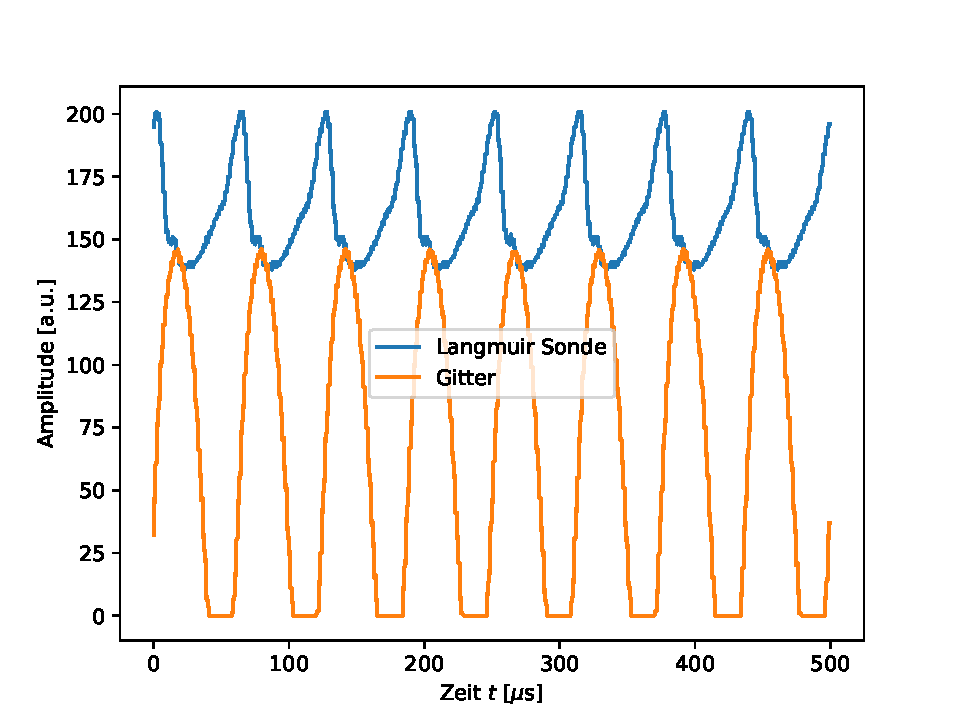
\includegraphics[scale=0.6]{oszi_3.pdf}
\caption{Die angelegte Spannung am Gitter und das gemessene Signal mit der Langmuir-Sonde.}
\label{fig:oszi_3}
\end{figure}
\subsection{Plasma Kriterien}
In diesem Kapitel soll geprüft werden, ob die Plasma Kriterien mit den berechnetern Werten erfüllt werden. Ein Kriterium ist, dass das gesamte System viel größer als die Debye-Länge $\lambda_{\mathrm{D}}$
\begin{align}
\lambda_{\mathrm{D}} = \sqrt{\frac{\epsilon_0 T}{e^2 n}}
\end{align}
ist, wobei $T$ die Temepratur und $n$ die Teilchendichte ist. Diese Größen sind in den vorangegangen Kapiteln berechnet worden. Für die Werte $n \approx 10^{15} $ und $T=3.1108\ \mathrm{eV} $ ergibt sich
\begin{align}
\lambda_{\mathrm{D}} = 2.351 \cdot 10^{-4}\ \mathrm{m}.
\end{align}
Diese Länge ist klein im Vergleich zur Größe des Doppel Plasma Apparates. Dieses Kriterium ist somit erfüllt.  Ein weiteres Kriterium ist, das die Teilchenanzahl in der Debye-Kugel groß sein muss. Diese Teilchenanzahl  $N$ kann aus der Debye-Länge $\lambda_{\mathrm{D}}= 2.351 \cdot 10^{-4}\ \mathrm{m}$ und der Dichte $n \approx 10^{15}$ berechnet werden
\begin{align}
N = V n= \frac{4}{3}\pi \lambda_{\mathrm{D}}^3 n = 54431.023 ,
\end{align}
wobei $V$ das Volumen der Deybe-Kugel ist. Das bedeutet, dass in der Debye Kugel ungefähr 54431 Teilchen sind. Das zweite Kriterium ist somit auch erfüllt. Das dritte Plasmakriterium ist, dass die Stoßzeit viel größer ist als die Periodendauer der Schwingungen des Plasmas. Die Stzoßzeit $\tau$ kann berechnet werden mit
\begin{align}
  \tau = \frac{1}{v \sigma n_0},
\end{align}
wobei $v$ die mittlere Geschwindigkeit der Elektronen, $\sigma$  der Streuquerschnitt und $n_0$ die Neutralteilchendichte ist. Für den Streuquerschnitt kann $\sigma= 5 \cdot 10^{-19}\ \mathrm{m}^2 $ angenommen werden, für die mittlere Geschwindigkeit gilt $v= \sqrt{2 T_{\mathrm{e}}/m_{\mathrm{e}}} $ und die Neutralteilchendichte $n_0=p/(k_{\mathrm{B}}T_{\mathrm{Gas}})$ kann mit dem idealem Gasgesetz berechnet werden. Aufgrund des defekten Druckmessgerätes ist der Druck in dem Doppel Plasma Apparat nicht bekannt. Deshalb kann die Überprüfung dieses Kriteriums nicht durchgeführt werden. Grundsätzlich müsste die berechnete Stoßzeit mit der Plasmafrequnz multilpiziert werden und das Ergebniss davon müsste viel größer als eins sein. 

